\section{What is Aging?}

\subsection{Definition and Hallmarks}

\begin{frame}[c]{Aging}
    \large

    \begin{block}{Definition \cite{sen2016epigenetic}}
        Aging is characterized by progressive decline in tissue and organ
        function and increased risk of mortality.
    \end{block}
    \pause
    But how can we measure it?
    \pnote{
        If someone remembers: ask me what aging is \\
        biologically, not enough time now
    }
\end{frame}


\begin{frame}[c]{Hallmarks of Aging: Measuring biological Age}
    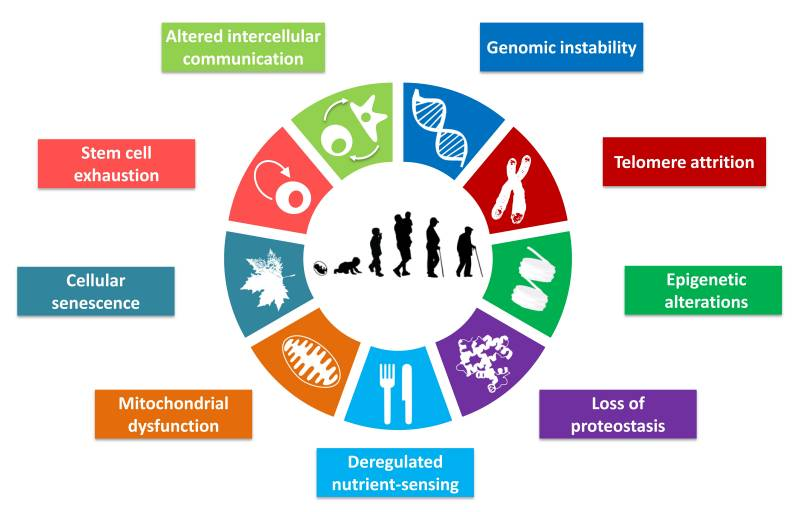
\includegraphics[width=\textwidth]{hallmarks_aging} \\
    \scriptsize
    Source: \cite{lopez2013hallmarks}
    \pnote{
        Groundbreaking paper, one of the most-cited \\
        Aging: accumulating damage to hallmark
        \par
        One hallmark also affects and damages others \\
        Each one has a theory of aging \\
        % Classified as Primary (causes), Antagonistic \\
        % (responses), Integrative (phenotype) \\
        % Unclear if actually the case \\
    }
    % maybe explain items better? re-use icons?
    % pretty central slide after
\end{frame}

